\documentclass[]{article}
\newcommand{\FileDepth}{../../..}
\usepackage[letterpaper, landscape, margin=0.5cm]{geometry}
\usepackage[T1]{fontenc}
\usepackage{textcomp}%Not strictly necessary, but gives \textmu command for "micro."
\usepackage{fancyhdr}
\usepackage{amsmath}
\usepackage{amssymb}
\usepackage{graphicx}
\usepackage{xcolor}
\usepackage{tikz}
\usetikzlibrary{calc}
\usepackage[shortlabels]{enumitem}
\usepackage{multicol}
\usepackage{vwcol}
\usepackage{hyperref}
\usepackage{wrapfig}
%opening
\newcommand{\SecType}{L}
\newcommand{\Week}{7}
\title{PH 211 Lecture \Week}
\author{Benjamin Bauml}
\date{Summer 2024}

\newcommand{\Purpose}{4}
\newcommand{\DefOnly}{0}

\input{\FileDepth/Formats/Assignment20240614.tex}
\usepackage[absolute]{textpos}
% This package relies on Assignment Format 2024-06-14 or later to work. It is recommended that the Purpose and DefOnly commands be given as such:
%\newcommand{\Purpose}{4}
%\newcommand{\DefOnly}{0}
% Activities need to be entered outside of the TeacherMargin and PresentSpace environments, otherwise they will be defined only locally. They can even go in the preamble.
\newenvironment{TeacherMargin}{\begin{textblock*}{10.8cm}(0.5cm,0.5cm)
\small}{\end{textblock*}
\hspace{0.1cm}}
\newenvironment{PresentSpace}{\begin{textblock*}{0.3cm}(26.85cm,9.35cm)
--
\end{textblock*}
\begin{textblock*}{15.6cm}(11.8cm,0.5cm)
\begin{Repurpose}{1}
\Large}{\end{Repurpose}
\end{textblock*}
\hspace{0.1cm}}

%\newcommand{\FBDaxes}[4][2]{
	\begin{scope}[shift={(#2)},rotate=#3]
		% x-axis
		\draw[thick,->] (-#1,0) -- (#1,0);
		\node[anchor=west] at (#1,0) {$x$};
		% y-axis
		\draw[thick,->] (0,-#1) -- (0,#1);
		\node[anchor=south] at (0,#1) {$y$};
		\coordinate (#4) at (0,0);
	\end{scope}
}
\newcommand{\FBDvectorMA}[4]{
	\begin{scope}[shift={(#1)}]
		\coordinate (#4tip) at ({#2*cos(#3)},{#2*sin(#3)});
		\draw[ultra thick,blue,->] (#1) -- (#4tip);
	\end{scope}
}
\newcommand{\FBDvectorXY}[3]{
	\begin{scope}[shift={(#1)}]
		\coordinate (#3tip) at (#2);
		\draw[ultra thick,blue,->] (0,0) -- (#3tip);
	\end{scope}
}
\newcommand{\FBDdot}[1]{
	\filldraw[black] (#1) circle (3pt);
}
\newcommand{\FBDbox}[5][1]{
	\begin{scope}[shift={(#2)},rotate=#3]
		\filldraw[color=black,fill=white,thick] ({-#1/2},{#1/2}) -- ({-#1/2},{-#1/2}) -- ({#1/2},{-#1/2}) -- ({#1/2},{#1/2}) -- cycle;
		% Left side coordinates
		\coordinate (#4ltq) at ({-#1/2},{#1/4});
		\coordinate (#4lcent) at ({-#1/2},0);
		\coordinate (#4lbq) at ({-#1/2},{-#1/4});
		% right side coordinates
		\coordinate (#4rtq) at ({#1/2},{#1/4});
		\coordinate (#4rcent) at ({#1/2},0);
		\coordinate (#4rbq) at ({#1/2},{-#1/4});
		% top coordinates
		\coordinate (#4tlq) at ({-#1/4},{#1/2});
		\coordinate (#4tcent) at (0,{#1/2});
		\coordinate (#4trq) at ({#1/4},{#1/2});
		% bottom coordinates
		\coordinate (#4blq) at ({-#1/4},{-#1/2});
		\coordinate (#4bcent) at (0,{-#1/2});
		\coordinate (#4brq) at ({#1/4},{-#1/2});
		% corners
		\coordinate (#4tl) at ({-#1/2},{#1/2});
		\coordinate (#4tr) at ({#1/2},{#1/2});
		\coordinate (#4bl) at ({-#1/2},{-#1/2});
		\coordinate (#4br) at ({#1/2},{-#1/2});
		\node at (0,0) {#5};
	\end{scope}
}
%\newcommand{\MVec}[3][0]{%Creates a momentum vector of length #3 centered at #2 and rotated #1 degrees counterclockwise.
	\begin{scope}[rotate=#1,shift={(#2)}]
		\draw[->,thick] ({-#3/2},0) -- ({#3/2},0);
	\end{scope}
}
\newcommand{\MDot}[1]{%Creates a dot at #1 to represent a zero vector.
	\filldraw (#1) circle (1pt);
}
\newcommand{\MVDRows}[2][4.5]{%Creates the rows (initial, delta, final) of a momentum vector diagram. The optional argument determines the width of the table, and defaults to a good length for three columns (two objects and the total system). The non-optional argument gives a coordinate name (not displayed) to the diagram.
	\begin{scope}
		%\draw[thick] (0,5.5) -- (0,0);
		\draw[thick] (-1,4.5) -- (#1,4.5);
		\node at (-0.5,3.75) {$\vec{p}_{i}$};
		\draw[thick] (-1,3) -- (#1,3);
		\node at (-0.5,2.25) {$\Delta\vec{p}$};
		\draw[thick] (-1,1.5) -- (#1,1.5);
		\node at (-0.5,0.75) {$\vec{p}_{f}$};
		\coordinate (#2) at (0,5);
	\end{scope}
}
\newcommand{\MVDCol}[4][0.75]{%Creates a column for an object in a momentum vector diagram. The first (non-optional) argument is the coordinate name (not displayed) of the column, while the second is the displayed column header. The first argument also names the three entries down the column. The third argument anchors the column, so it should either be the coordinate name of the MVD (for the first column) or the coordinate name of the previous column. The optional argument indicates how far the center of the column should be from the previous column's edge, and defaults to 0.75.
	\begin{scope}[shift={(#4)}]
		\node at (#1,0) {#3};
		%\draw[thick] ({#1*2},0.5) -- ({#1*2},-5);
		\draw[thick] (0,0.5) -- (0,-5);
		\coordinate (#2init) at (#1,-1.25);
		\coordinate (#2delt) at (#1,-2.75);
		\coordinate (#2fin) at (#1,-4.25);
		\coordinate (#2) at ({#1*2},0);
	\end{scope}
}

%\input{\FileDepth/Activities/Activity_One/Activity_One.tex}
%\input{\FileDepth/Activities/Activity_Two/Activity_Two.tex}

\begin{document}
\begin{TeacherMargin}

\end{TeacherMargin}
\begin{PresentSpace}
\begin{center}
	\huge Lecture 7: Projectile Motion II
\end{center}
\vspace{-0.3cm}
\underline{Announcements}
\begin{itemize}
	\item Group Expectations are due at 8pm tonight.
	\begin{itemize}
		\item Only one submission per group.
		\item Fill out the form even if you don't have a group. I will use it to assign you.
	\end{itemize}
	\item Project Proposal is due on Friday.
	\begin{itemize}
		\item Not released yet (will be after I form the groups in Canvas).
		\item Decide on a topic and a format with your group.
	\end{itemize}
	\item Make sure you can see your feedback on homework, labs, and Get-Ready assignments!
\end{itemize}
\end{PresentSpace}
\newpage
\begin{TeacherMargin}
	\noindent\textbf{1a) Understand the Problem}
	\begin{itemize}
		\item Known:
		\begin{itemize}
			\item $v_{0}=25$ m/s, $\theta = 45^{\circ}$
			\item By assumption: $\vec{a}=+g\hat{y}$, $g\approx9.8$ m/s$^{2}$
		\end{itemize}
		\item Unknown:
		\begin{itemize}
			\item $\Delta x$ (horizontal distance traveled), $\Delta y$ (vertical distance traveled), $t_{f}$ (time of flight), $v_{f}$ final speed
		\end{itemize}
	\end{itemize}
	\noindent\textbf{1b) Identify Assumptions}
	\begin{itemize}
		\item The mountain has a perfectly smooth slope, and the arrow will not travel far enough to reach the bottom.
		\begin{itemize}
			\item While mountains are not really this smooth, this assumption reflects the picture, and makes it easier to mathematically describe the slope.
			\item Mountains are really tall, and reaching the base of the mountain would complicate the problem.
		\end{itemize}
		\item The arrow is not affected by moving through air.
		\begin{itemize}
			\item An arrow is fast and aerodynamic, and we don't really know how to handle air resistance or the effects of wind, so we should ignore these effects to make the problem solvable.
		\end{itemize}
		\item Near Earth's surface ($g\approx9.8$ m/s$^{2}$)
		\begin{itemize}
			\item So far, all known archery occurs on Earth, and though we are farther up on this mountain, the arrow won't fall so far that the variations in gravity are significant.
		\end{itemize}
		\item $\vec{a}=+g\hat{y}$
		\begin{itemize}
			\item Since the object is in free-fall with no wind or air effects, and it isn't traveling far enough for the curvature of the Earth to matter, acceleration is straight down and purely gravitational.
		\end{itemize}
	\end{itemize}
	\noindent\textbf{1c) Represent Physically} \\
	Choosing $\hat{y}$ pointing down saves us a few negative signs in the process of the solution.
	\begin{center}
		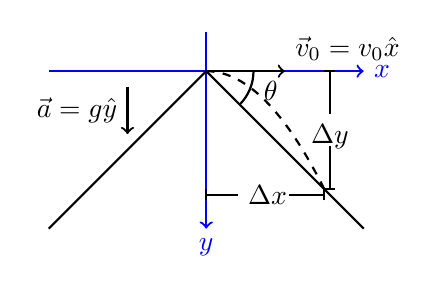
\begin{tikzpicture}
			\begin{scope}
				\draw[blue,thick,<->] (0,-2) node[anchor=north] {$y$} -- (0,0) -- (2,0) node[anchor=west] {$x$};
				\draw[blue,thick] (0,0.5) -- (0,0) -- (-2,0);
				\draw[thick] (-2,-2) -- (0,0) -- (2,-2);
				\draw[thick,->] (0,0) -- (1,0) node[anchor=south west] {$\vec{v}_{0} = v_{0}\hat{x}$};
				\draw[thick] (0.6,0) node[anchor=north west] {$\theta$} arc (0:-45:0.6);
				\begin{scope}[shift={(1.5,0)}]
					\draw[thick] (0,0) -- (4pt,0) (2pt,0) -- (2pt,-0.55) node[anchor=north] {$\Delta y$} (2pt,-0.95) -- (2pt,-1.5) (0,-1.5) -- (4pt,-1.5);
				\end{scope}
				\begin{scope}[shift={(0,-1.5)}]
					\draw[thick] (0,0) -- (0,-4pt) (0,-2pt) -- (0.4,-2pt) node[anchor=west] {$\Delta x$} (1.05,-2pt) -- (1.5,-2pt) (1.5,-4pt) -- (1.5,0);
				\end{scope}
				\draw[thick,->] (-1,-0.2) -- (-1,-0.5) node[anchor=east] {$\vec{a}=g\hat{y}$} -- (-1,-0.8);
				\draw[thick,dashed,domain=0:1.5,variable=\x] plot (\x,{-2*\x*\x/3});
			\end{scope}
		\end{tikzpicture}
	\end{center}
\end{TeacherMargin}
\begin{PresentSpace}
	\vspace{-10pt}
	\section*{L7-1: Archer of the Peak}
	\vspace{-10pt}
	You (still a long-distance archer) move to the top of the mountain below. The initial speed of your arrow is now 25.0 m/s, and you release it horizontally to the right. Following the steps for solving an A*R*C*S problem, find where the arrow lands.
	\begin{itemize}
		\item \textit{Hint 1:} You will still need to set up separate equations for the $x$- and $y$-directions.
		\item \textit{Hint 2:} You can also relate the horizontal and vertical distances the arrow moves before striking the ground.
	\end{itemize}
	\begin{center}
		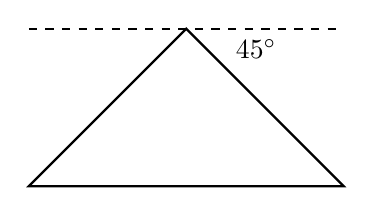
\begin{tikzpicture}
			\draw[thick,dashed] (-2,0) -- (2,0);
			\draw[thick] (-2,-2) -- (0,0) node[anchor=north west,shift={(0.5,0)}] {$45^{\circ}$} -- (2,-2) -- cycle;
		\end{tikzpicture}
	\end{center}
	\begin{center}
		\includegraphics[scale=0.4]{AnalyzeAndRepresent}
		%\includegraphics[scale=0.4]{Calculate}
		%\includegraphics[scale=0.4]{Sensemake}
	\end{center}
\end{PresentSpace}
\newpage
\begin{TeacherMargin}
	\noindent\textbf{2a) Represent Principles}
	
	\noindent 2-D Kinematics: {\color{blue}Known} {\color{red}Unknown} {\color{purple}Wanted}
	\begin{align*}
		{\color{purple}\Delta x} & = {\color{blue}v_{0x}}{\color{red}t_{f}} + \frac{1}{2}{\color{blue}a_{x}}{\color{red}t_{f}}^{2} & {\color{red}\Delta y} & = {\color{blue}v_{0y}}{\color{red}t_{f}} + \frac{1}{2}{\color{blue}a_{y}}{\color{red}t_{f}}^{2} \\
		{\color{red}v_{fx}} & = {\color{blue}v_{0x}} + {\color{blue}a_{x}}{\color{red}t_{f}} & {\color{red}v_{fy}} & = {\color{blue}v_{0y}}+{\color{blue}a_{y}}{\color{red}t_{f}} \\
		{\color{red}v_{fx}}^{2} & = {\color{blue}v_{0x}}^{2} + 2{\color{blue}a_{x}}{\color{purple}\Delta x} & {\color{red}v_{fy}}^{2} & = {\color{blue}v_{0y}}^{2} + 2{\color{blue}a_{y}}{\color{red}\Delta y}
	\end{align*}
	We can avoid the bottom four equations, since we don't really want to know $v_{f}$. \\
	Trigonometry: $\tan{\color{blue}\theta} = \frac{\color{red}\Delta y}{\color{purple}\Delta x}$ \\
	\textbf{2b) Find Unknown(s) Symbolically} \\
	Between ${\color{purple}\Delta x} = {\color{blue}v_{0x}}{\color{red}t_{f}} + \frac{1}{2}{\color{blue}a_{x}}{\color{red}t_{f}}^{2}$ and ${\color{red}\Delta y} = {\color{blue}v_{0y}}{\color{red}t_{f}} + \frac{1}{2}{\color{blue}a_{y}}{\color{red}t_{f}}^{2}$, we have three unknowns ($t_{f},\ \Delta x,\ \Delta y$). However, we can bring in our one trigonometric equation to relate two of the unknowns, giving us a solvable system of three equations.
	\begin{align*}
		{\color{purple}\Delta x} & = {\color{blue}v_{0x}}{\color{red}t_{f}} + \frac{1}{2}{\color{blue}a_{x}}{\color{red}t_{f}}^{2} & {\color{red}\Delta y} & = {\color{blue}v_{0y}}{\color{red}t_{f}} + \frac{1}{2}{\color{blue}a_{y}}{\color{red}t_{f}}^{2} \\
		\Delta x & = v_{0}t_{f} & \Delta y & = \frac{1}{2}gt_{f}^{2}
	\end{align*}
	\[
	\tan\theta = \frac{\Delta y}{\Delta x} = \frac{\frac{1}{2}gt_{f}^{2}}{v_{0}t_{f}} = \frac{g}{2v_{0}}t_{f} \implies t_{f} = \frac{2v_{0}}{g}\tan\theta
	\]
	\begin{align*}
	\Delta x & = \frac{2v_{0}^{2}}{g}\tan\theta & \Delta y & = \frac{2v_{0}^{2}}{g}\tan^{2}\theta
	\end{align*}
	\textbf{2c) Plug in Numbers} \\
	I will actually use $g\approx10$ m/s$^{2}$ for simplicity here:
	\[
	\Delta x \approx \frac{2(25\text{ m/s})^{2}}{10\text{ m/s}^{2}}\tan(45^{\circ}) = 125\text{ m}.
	\]
\end{TeacherMargin}
\begin{PresentSpace}
	\vspace{-10pt}
	\section*{L7-1: Archer of the Peak}
	\vspace{-10pt}
	You (still a long-distance archer) move to the top of the mountain below. The initial speed of your arrow is now 25.0 m/s, and you release it horizontally to the right. Following the steps for solving an A*R*C*S problem, find where the arrow lands.
	\begin{itemize}
		\item \textit{Hint 1:} You will still need to set up separate equations for the $x$- and $y$-directions.
		\item \textit{Hint 2:} You can also relate the horizontal and vertical distances the arrow moves before striking the ground.
	\end{itemize}
	\begin{center}
		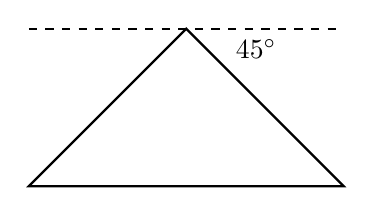
\begin{tikzpicture}
			\draw[thick,dashed] (-2,0) -- (2,0);
			\draw[thick] (-2,-2) -- (0,0) node[anchor=north west,shift={(0.5,0)}] {$45^{\circ}$} -- (2,-2) -- cycle;
		\end{tikzpicture}
	\end{center}
	\begin{center}
		%\includegraphics[scale=0.4]{AnalyzeAndRepresent}
		\includegraphics[scale=0.4]{Calculate}
		%\includegraphics[scale=0.4]{Sensemake}
	\end{center}
\end{PresentSpace}
\newpage
\begin{TeacherMargin}
	\noindent\textbf{3a) Units} \\
	We want $[\Delta x] = \text{m}$, and we know $[v_{0}]=\frac{\text{m}}{\text{s}}$, $[g]=\frac{\text{m}}{\text{s}^{2}}$, and both $[\tan(\theta)]=1$ and $[2]=1$ (unitless), so
	\[
	[\Delta x] = \frac{[2][v_{0}]^{2}}{[g]}[\tan\theta] = \frac{\text{m}^{2}/\text{s}^{2}}{\text{m/s}^{2}} = \text{m}
	\]
	\textbf{3b) Numbers} \\
	$\Delta x$ and $\Delta y$ are both 125 m, and $\sqrt{\Delta x^{2}+\Delta y^{2}} = 125\sqrt{2}\text{ m} \approx 176$ m, which is comparable to the distance we shot in L6-2: Long-Distance Archer. We achieved it at a lower speed here, since our arrow could fall toward its target (rather than having to keep itself above flat ground for the entire flight). \\
	\textbf{3c) Symbols}
	\begin{itemize}
		\item $v_{0}$ increases
		\begin{itemize}
			\item If it is shot faster, the arrow will have more horizontal speed and have farther to fall (and hence more time in flight), so it should achieve more horizontal distance.
			\item $\Delta x$ increases as $v_{0}$ increases, so our equation matches this prediction.
		\end{itemize}
		\item $g$ increases
		\begin{itemize}
			\item If $g$ increases (say we do archery on Jupiter), then the arrow will be dragged to the ground more quickly, so it will not travel as far.
			\item $\Delta x$ decreases as $g$ increases, so our equation matches this prediction.
		\end{itemize}
		\item $\theta=0^{\circ}$
		\begin{itemize}
			\item In this special case, there is no mountain, and an arrow launched horizontally at ground level will hit the ground immediately, having no range.
			\item $\Delta x = \frac{2v_{0}^{2}}{g}\tan(0^{\circ}) = 0$
		\end{itemize}
	\end{itemize}
\end{TeacherMargin}
\begin{PresentSpace}
	\vspace{-10pt}
	\section*{L7-1: Archer of the Peak}
	\vspace{-10pt}
	You (still a long-distance archer) move to the top of the mountain below. The initial speed of your arrow is now 25.0 m/s, and you release it horizontally to the right. Following the steps for solving an A*R*C*S problem, find where the arrow lands.
	\begin{itemize}
		\item \textit{Hint 1:} You will still need to set up separate equations for the $x$- and $y$-directions.
		\item \textit{Hint 2:} You can also relate the horizontal and vertical distances the arrow moves before striking the ground.
	\end{itemize}
	\begin{center}
		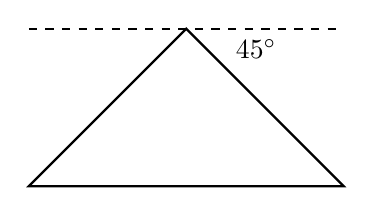
\begin{tikzpicture}
			\draw[thick,dashed] (-2,0) -- (2,0);
			\draw[thick] (-2,-2) -- (0,0) node[anchor=north west,shift={(0.5,0)}] {$45^{\circ}$} -- (2,-2) -- cycle;
		\end{tikzpicture}
	\end{center}
	\begin{center}
		%\includegraphics[scale=0.4]{AnalyzeAndRepresent}
		%\includegraphics[scale=0.4]{Calculate}
		\includegraphics[scale=0.4]{Sensemake}
	\end{center}
\end{PresentSpace}
\newpage
\begin{TeacherMargin}
	
\end{TeacherMargin}
\begin{PresentSpace}
	\section*{Main Ideas}
	\begin{itemize}
		\item We can use the kinematics equations to solve for any quantity of interest when the acceleration is constant.
		\item Motion in 2 dimensions can be broken down into independent motion in each dimension.
	\end{itemize}
\end{PresentSpace}
\end{document}